\newpage
\chapter{Sơ đồ Use case}\label{chap:UC}
\begin{figure}[!ht]
	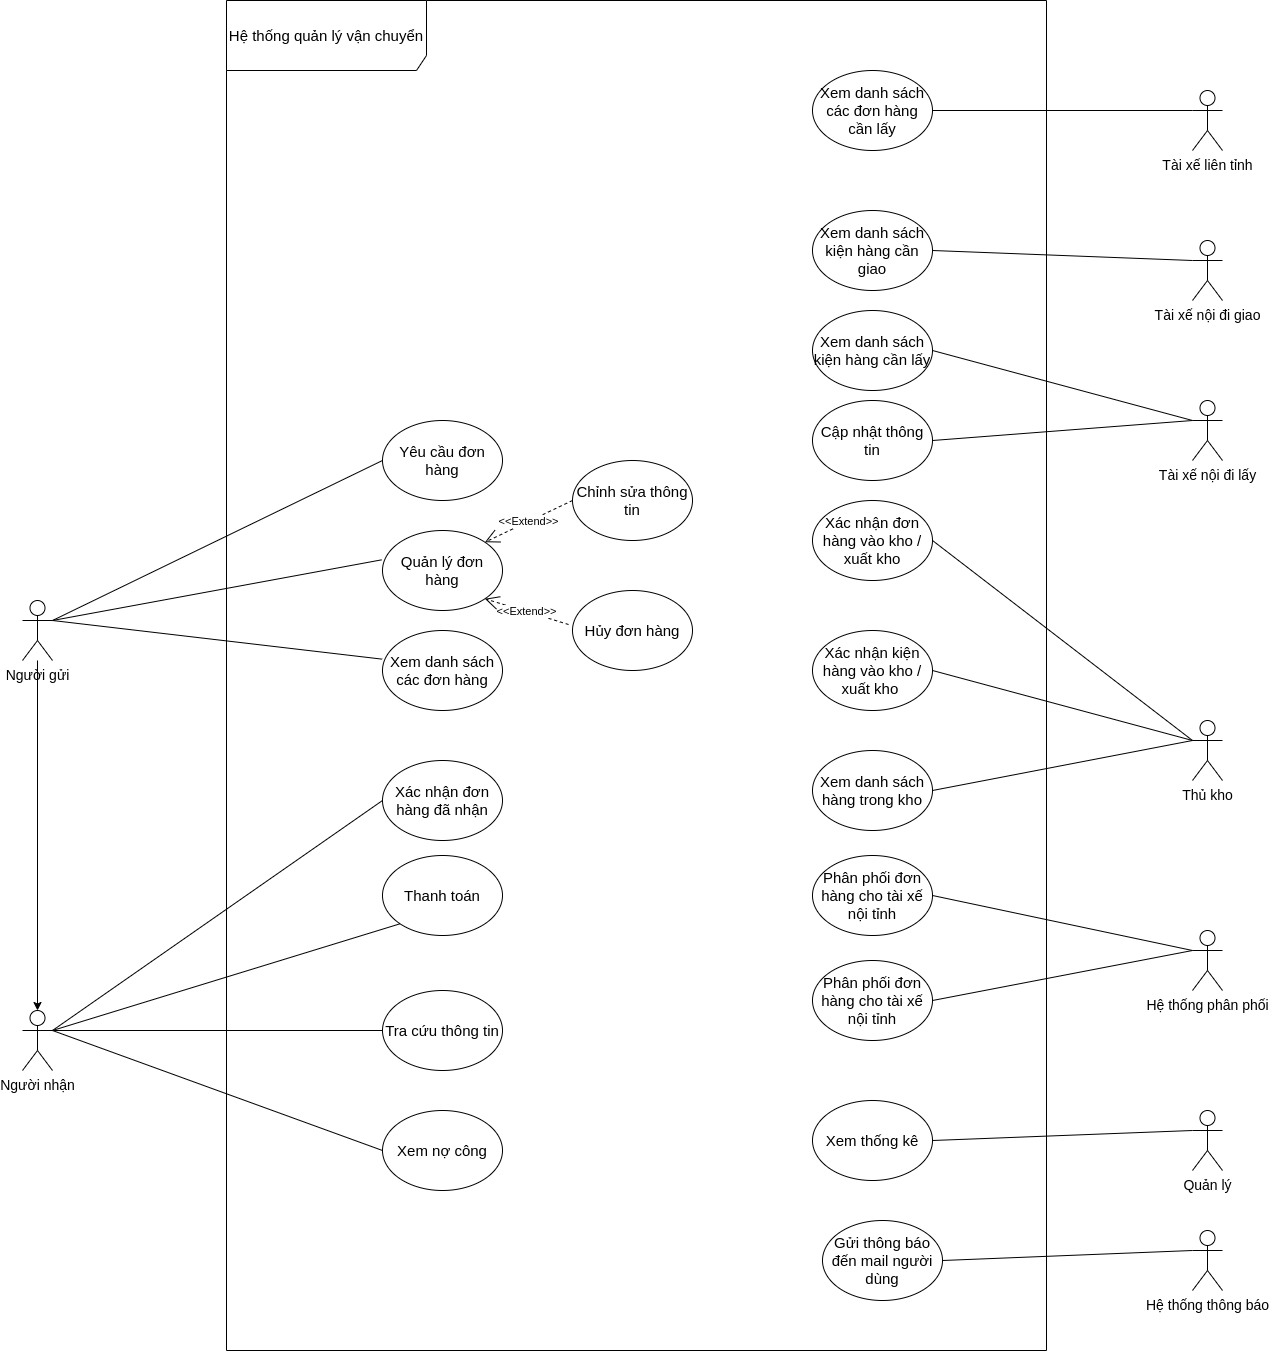
\includegraphics[width=1\textwidth]{/UseCase.png}
	\centering
	\linebreak
	\caption{Sơ đồ Use case}
\end{figure}

\newpage

\section{Đặc tả Use case}
\begin{itemize}
	\item 
	\subsection{Trạng thái đơn hàng}
	\begin{itemize}
		\item Đơn nháp: Trạng thái đầu, khi người dùng tạo yêu cầu đơn hàng
		\item Chờ bàn giao: Khi người dùng ấn nút gửi yêu cầu. Cho phép tối đa 30s để người dùng có thể chỉnh sửa hoặc hủy đơn (Có thể nhấn nút submit để chốt sớm hơn). Sau thời gian đó đơn hàng sẽ chuyển status sang trạng thái kế tiếp
		\item Trong hàng chờ phân phối: Đưa vào hàng chờ của hệ thống phân phối (Chi tiết ghi trong actor "Hệ thống phân phối")
		\item Đang lấy hàng: Các kiện hàng của đơn hàng đã và đang được đến lấy về kho (Có thông tin thêm là <x / tổng số kiện hàng> đã được lấy).
		\item Đã vào kho tập trung <Địa điểm 1>: Các kiện hàng của đơn hàng đã được lấy hết và được đưa vào kho <Địa điểm 1> 
		\item Đang giao liên tỉnh: Đơn hàng đã xuất kho 1 và đang được giao liên tỉnh từ kho 1 đến kho 2
		\item Đã vào kho tập trung <Địa điểm 2>: Các kiện hàng của đơn hàng đã được lấy hết và được đưa vào kho <Địa điểm 2>
		\item Đang giao hàng: Các kiện hàng của đơn hàng đã và đang được giao đến người nhận cuối
		\item Hoàn tất: Khi tất cả các kiện hàng của đơn hàng đã đến địa điểm cuối
		\item Đơn hủy: Trạng thái khi khách hàng hủy đơn ở trạng thái chờ bàn giao (Khách hàng chỉ được hủy ở trạng thái chờ bàn giao).
	\end{itemize}
	\subsection{Người gửi}
	\begin{itemize}
		\item \textbf{Tạo đơn hàng:} Người gửi cần điền những thông tin sau: 
		\begin{itemize}
			\item Bên gửi:
			\begin{itemize}
				\item Tên người gửi
				\item Số điện thoại
				\item Địa chỉ, chia làm 3 phần gồm Số địa chỉ + tên đường, Quận - Huyện, Phường - Xã. Quận - Huyện và Phường - Xã được nhập bằng cách chọn trong một dropdown có sẵn.
			\end{itemize}
			\item Bên nhận:
			\begin{itemize}
				\item Tên người nhận
				\item Số điện thoại
				\item Địa chỉ, tương tự như bên gửi.
			\end{itemize}
			\item Thông tin về (các) món hàng muốn gửi:
			\begin{itemize}
				\item Tên sản phẩm + số lượng (Mặc định là 1). Có thể thêm nhiều sản phẩm và có thể chỉnh sửa số lượng của từng sản phẩm đã thêm.
				\item Khối lượng (Để tính phí vận chuyển). Nhân viên đến lấy hàng sẽ tiến hành xác nhận bằng cách đo lại và sẽ yêu cầu khách hàng cập nhật lại khối lượng nếu như khối lượng đã nhập trước đó là không chính xác.
				
			\end{itemize}
			\item Lựa chọn cho bên nhận:
			\begin{itemize}
				\item Không cho xem hàng.
				\item Cho xem hàng nhưng không cho thử.
				\item Cho thử hàng.
			\end{itemize}
			\item Lựa chọn tính phí cho bên gửi hoặc bên nhận 
			\item Lựa chon gửi hàng / nhận hàng tại kho sẽ không tính phí nội tỉnh(phí liên tỉnh luôn có ). Ngược lại sẽ tính phí nội tỉnh (gửi và nhận giống nhau). 
			\item Hệ thống sẽ tự tính cước vận chuyển dựa trên khoảng cách bên gửi/nhận và khối lượng món hàng.
			\item Các thông tin ghi chú khác (Người gửi tự điền vào ô textbox).
			\item Mockup / Wireframe (Dự kiến tham khảo thiết kế UI của GHN):
		\end{itemize} 
		
		\begin{figure}[!ht]
			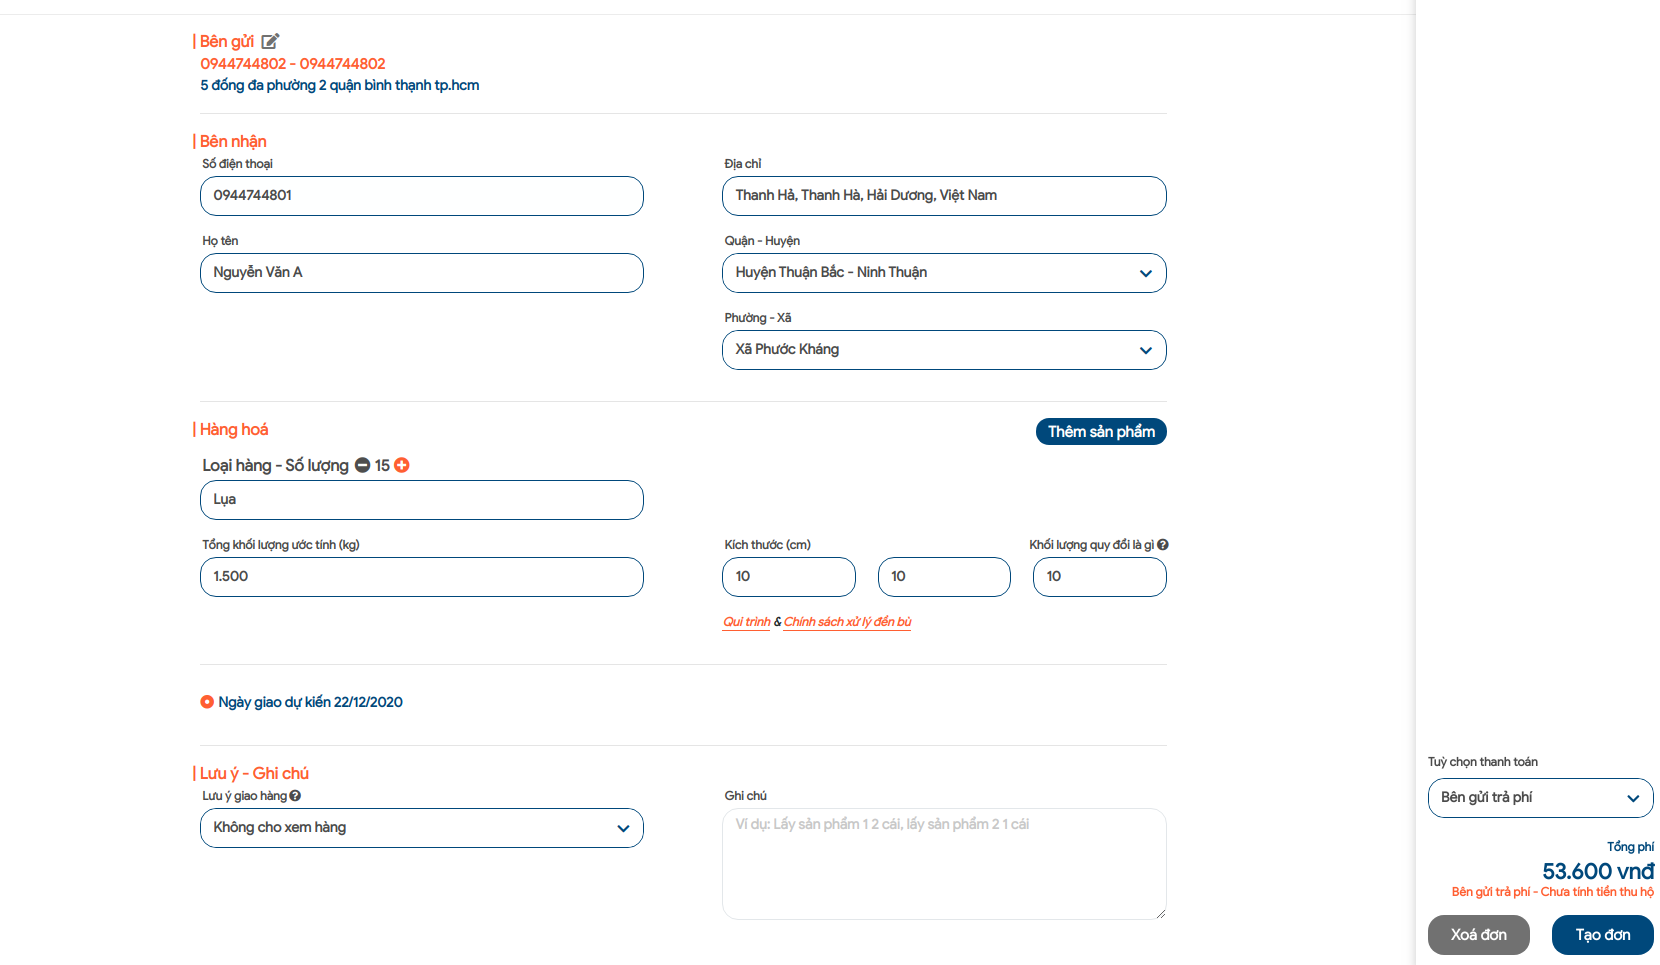
\includegraphics[width=1\textwidth]{/create-order.png}
			\centering
			\linebreak
			\caption{Giao diện tạo đơn hàng (dự kiến)}
		\end{figure}
		
		\item \textbf{Chỉnh sửa thông tin đơn hàng:} Nếu vẫn đang trong quá trình bàn giao và xác nhận(trong trạng thái \textbf{Chờ bàn giao}), người gửi có thể chỉnh sửa thông tin đơn hàng (Thông tin như trong mục tạo đơn, sẽ có giới hạn thông tin được chỉnh sửa).
		
		\item \textbf{Hủy đơn hàng:} Nếu vẫn đang trong quá trình bàn giao và xác nhận(trong trạng thái \textbf{Chờ bàn giao}), người gửi có thể hủy đơn hàng. Đơn hàng bị hủy sẽ được chuyển vào mục thùng rác và cho phép người dùng tái sử dụng thông tin của đơn hàng bị hủy ấy (Tạo lại đơn hàng mới dựa trên thông tin đơn hàng bị xóa ấy).
		
		\item \textbf{Xem danh sách các đơn hàng}: Các đơn hàng sẽ được chia theo trạng thái đã định nghĩa ở trên và người gửi có thể xem list các đơn hàng lọc theo trạng thái đó. Mockup / Wireframe (Dự kiến tham khảo thiết kế UI của GHN):
		
		\begin{figure}[!ht]
			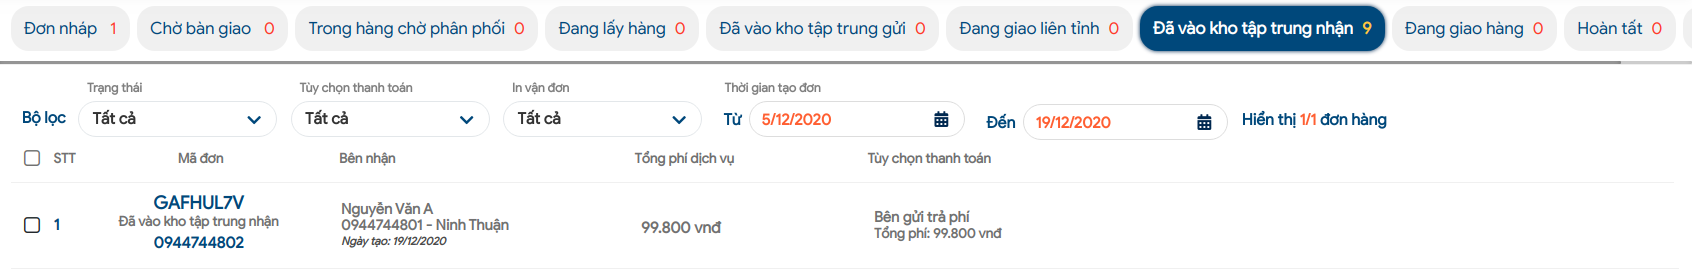
\includegraphics[width=1\textwidth]{/order-status.png}
			\centering
			\linebreak
			\caption{Giao diện xem danh sách các đơn hàng (dự kiến)}
		\end{figure}
		
		\item \textbf{Xem nợ công và thanh toán}: Do phí có thể được tính cho người gửi hoặc người nhận (theo nhu cầu của người gửi), người gửi và người nhận đều có thể xem nợ công và thực hiện thanh toán. Thanh toán dự định sẽ được thực hiện qua ZaloPay
	\end{itemize}
	
	\subsection{Người nhận}
	\begin{itemize}
		\item \textbf{Xem nợ công và thanh toán}: Tương tự UC của người gửi
		
		\item \textbf{Tra cứu thông tin đơn hàng:} Mỗi đơn hàng được tạo sẽ có một mã riêng biệt dùng cho người gửi/nhận tra cứu thông tin và tình trạng hiện tại của đơn hàng. Mockup / Wireframe (Dự kiến tham khảo thiết kế UI của GHN): 
		
		\begin{figure}[!ht]
			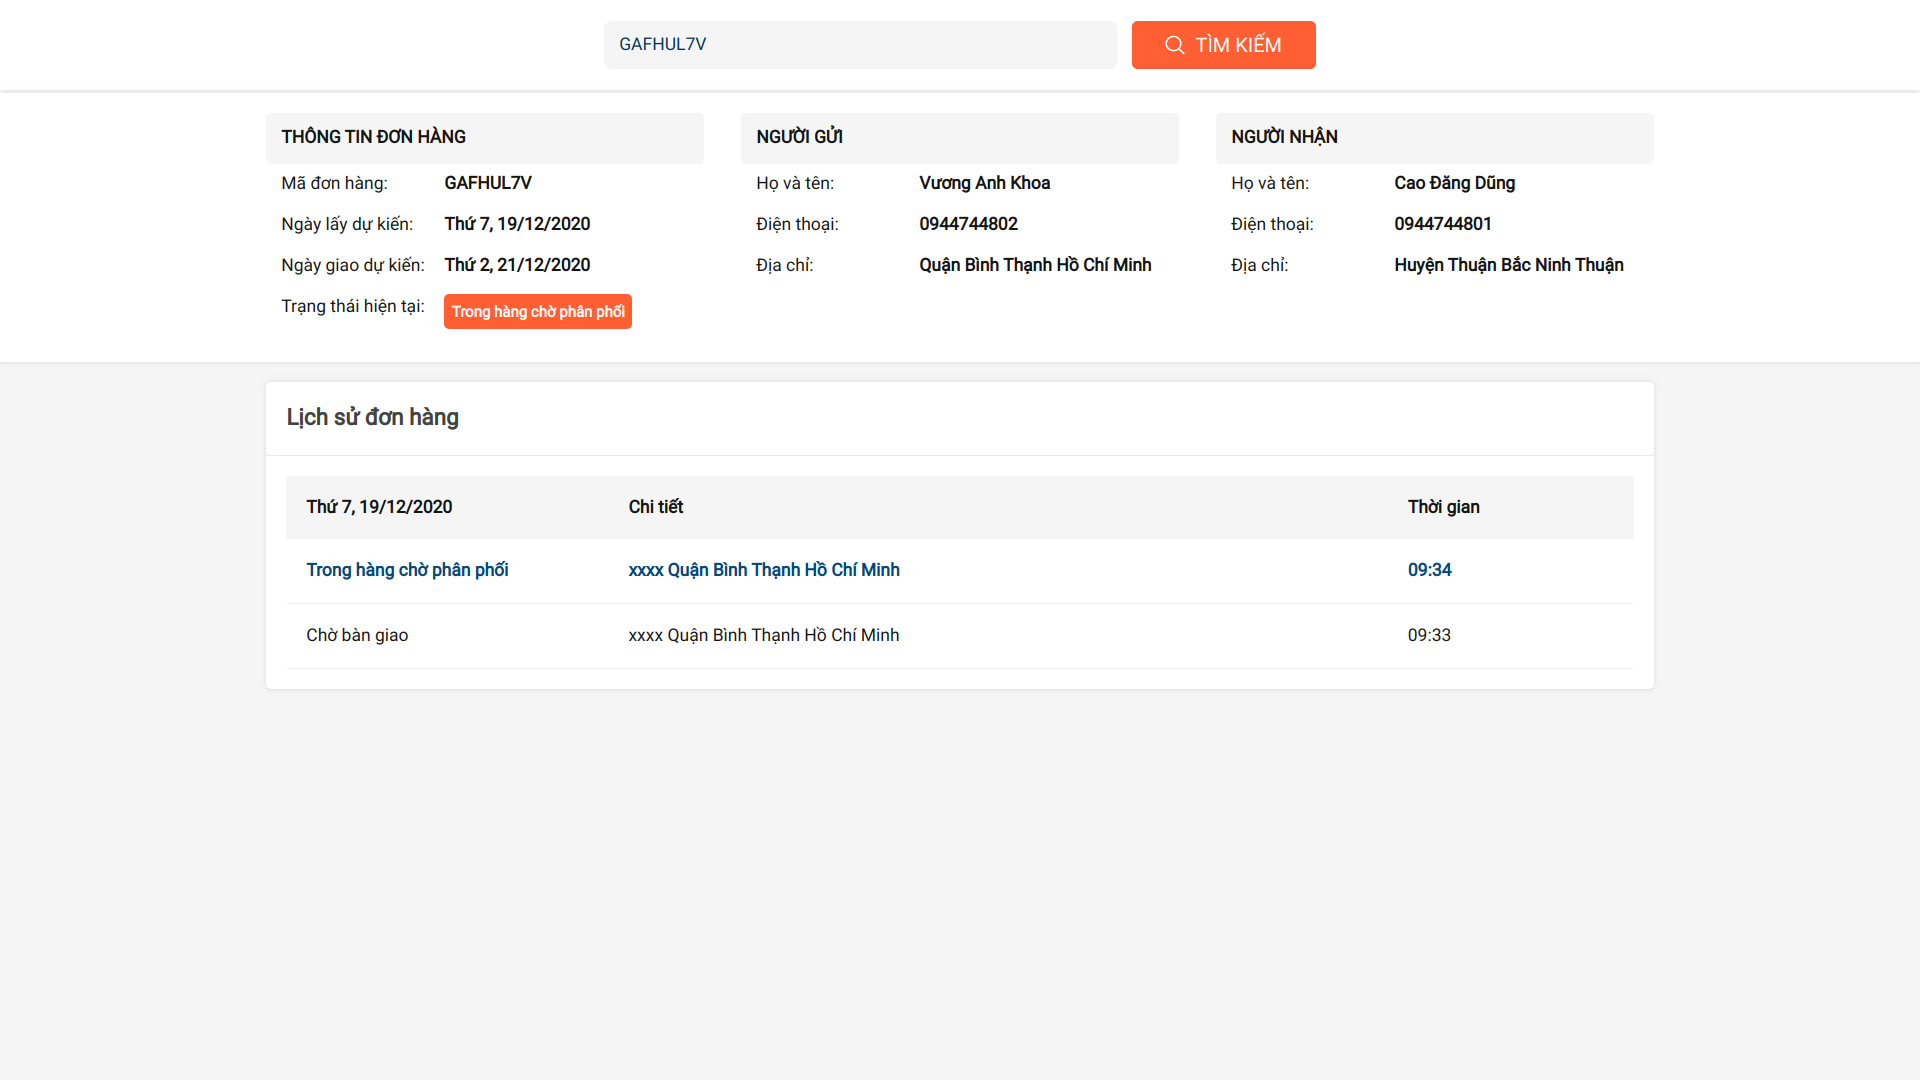
\includegraphics[width=0.95\textwidth]{/tracking.png}
			\centering
			\linebreak
			\caption{Giao diện theo dõi tình trạng đơn hàng (dự kiến)}
		\end{figure}
		
		\item \textbf{Xác nhận đơn hàng đã nhận}: Người nhận sẽ check vào những kiện hàng sẽ được nhận (trong đơn hàng của người nhận) có trong xe hoặc trong kho (nếu lựa là người nhận tự đến lấy). Nếu tất cả kiện hàng ở trong đơn hàng đã được check thì trạng thái đơn hàng cập nhật từ (Đang giao hàng -> Hoàn tất). Trong trường hợp nếu người nhận tự đến lấy thì sẽ có thêm khoản phí lưu kho (Được tính theo khoảng thời gian từ lúc đơn hàng nhập kho đến khi người nhận đến lấy).
	\end{itemize}
	
	\subsection{Tài xế nội tỉnh đi lấy}
	\begin{itemize}
		\item \textbf{Xem danh sách kiện hàng cần lấy:} Tài xế nội tỉnh sẽ được assign những kiện hàng cần đi lấy để thu gom về kho. Tài xế nội tỉnh có thể xem những thông tin cần thiết để tiến hành xử lí vận chuyển list danh sách các kiện hàng đó.
		
		\begin{figure}[!ht]
			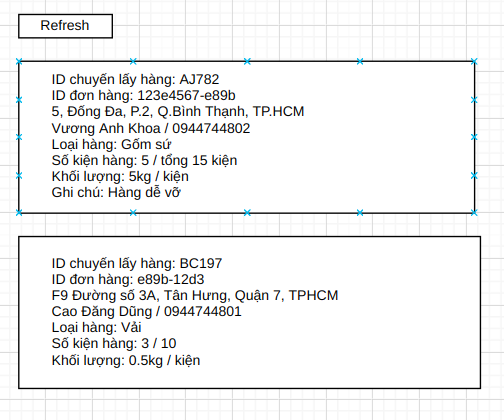
\includegraphics[width=0.7\textwidth]{/ntlay.png}
			\centering
			\linebreak
			\caption{Wireframe list các kiện hàng cần lấy của tài xế (dự kiến)}
		\end{figure}
		
		\item \textbf{Cập nhật nếu có thông tin sai sót}: Tài xế đến lấy hàng sẽ tiến hành đo lại và cập nhật thông tin kiện hàng nếu thông tin kiện hàng có sai sót (Như khối lượng, kích thước vv...). Sau đó, khách hàng sẽ tiến hành xác nhận lại thông tin tài xế cập nhật là chính xác để tiến hành giao nhận.
		
		\newpage
		
		\begin{figure}[!ht]
			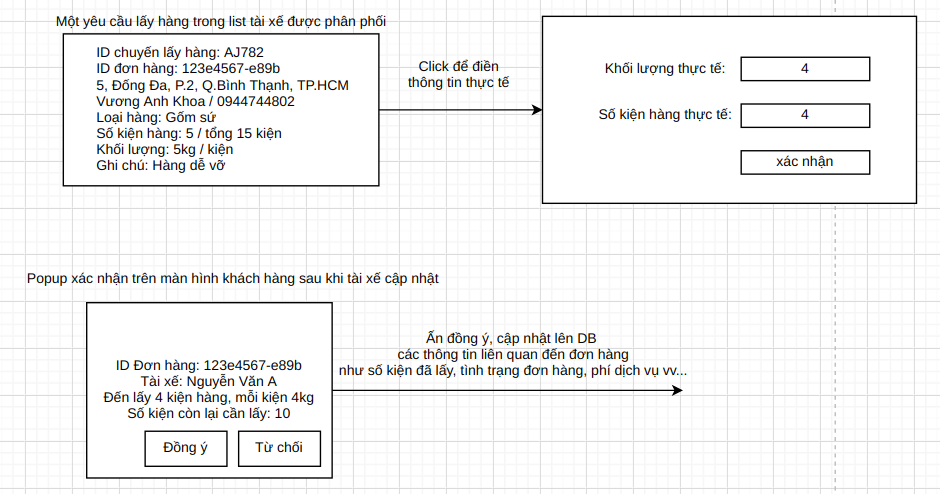
\includegraphics[width=1\textwidth]{/reconfirm.png}
			\centering
			\linebreak
			\caption{Wireframe miêu tả qui trình xác nhận thông tin sai sót}
		\end{figure}
	\end{itemize}
	
	\subsection{Tài xế nội tỉnh đi giao}
	\textbf{Xem danh sách kiện hàng cần giao}:  Tài xế nội tỉnh sẽ được assign những kiện hàng cần được giao cho người nhận. Tài xế nội tỉnh có thể xem những thông tin cần thiết để tiến hành xử lí vận chuyển list danh sách các kiện hàng đó.
	
	\subsection{Tài xế liên tỉnh} 
	\textbf{Xem danh sách kiện hàng cần lấy}: Tài xế liên tỉnh sẽ được assign những đơn hàng cần đi lấy để vận chuyển đến kho liên tỉnh. Tài xế liên tỉnh có thể xem những thông tin cần thiết để tiến hành xử lí vận chuyển list danh sách các đơn hàng đó.
	\subsection{Hê thống phân phối}
	\begin{itemize}
		\item \textbf{Phân phối đơn hàng cho tài xế nội tỉnh}: Các đơn hàng sẽ được đưa vào 2 loại hàng chờ (nội tỉnh): Hàng chờ hôm nay và hàng chờ các đơn hàng cho ngày hôm sau. Hệ thống qui định những kiện hàng được tạo trước <6h> tối sẽ được đưa vào hàng chờ hôm nay, còn những kiện hàng được tạo sau <6h> tối sẽ được đưa vào hàng chờ ngày hôm sau. Hệ thống sẽ chỉ phân phối các kiện hàng trong hàng chờ ngày hôm nay cho các tài xế nội tỉnh. Nếu hàng chờ ngày hôm nay chưa xử lí hết các kiện hàng thì sẽ được đẩy qua ngày hôm sau.Đơn vị ở đây là kiện hàng do xe nội tỉnh thường có kích thước nhỏ, không thể lấy hết cả 1 đơn hàng mà chỉ có thể lấy một số kiện hàng từ đơn ấy. Hệ thống sẽ cập nhật trạng thái từ <Trong hàng chờ phân phôi>  -->  <Đang lấy hàng>
		\item \textbf{Phân phối đơn hàng cho tài xế liên tỉnh}: Đơn hàng đã được tập kết đầy đủ (Tức toàn bộ kiện hàng của đơn hàng đã đến kho) sẽ được đưa vào hàng chờ liên tỉnh. Hệ thống qui định những đơn hàng đã được tập kết trước <12h> đêm sẽ được đưa vào hàng chờ hôm nay, còn những đơn hàng được tập kết sau <12h> đêm sẽ được đưa vào hàng chờ ngày hôm sau. Hệ thống sẽ chỉ phân phối các đơn hàng trong hàng chờ ngày hôm nay cho các tài xế liên tỉnh. Nếu hàng chờ ngày hôm nay chưa xử lí hết các đơn hàng thì sẽ được đẩy qua ngày hôm sau. Đơn vị ở đây là đơn hàng do xe liên tỉnh thường có kích thước lớn nên có thể chở cả 1 hoặc nhiều đơn hàng.
	\end{itemize}
	
	\subsection{Quản lí}
	
	\textbf{Xem thống kê}: Người quản lý có thể  xem thống kê về số lương đơn hàng trong tuần, tháng, năm thông qua biểu đồ; xem thống kê hiệu suất làm việc của tài xế ; số đơn hàng giao thành công và đơn hàng bị hủy trong tuần, tháng, năm.
	
	
	\subsection{Thủ kho}
	\begin{itemize}
		\item \textbf{Xem danh sách hàng trong kho}: Thủ kho sẽ xem list các đơn hàng có trong kho (Lọc theo tiêu chí tất cả, đơn hàng mà các kiện đã vào đủ, đơn hàng mà các kiện chưa vào đủ). Thông tin từng đơn hàng là loại hàng, <số kiện hàng đã vào kho / tổng số kiện>. 
		
		\begin{figure}[!ht]
			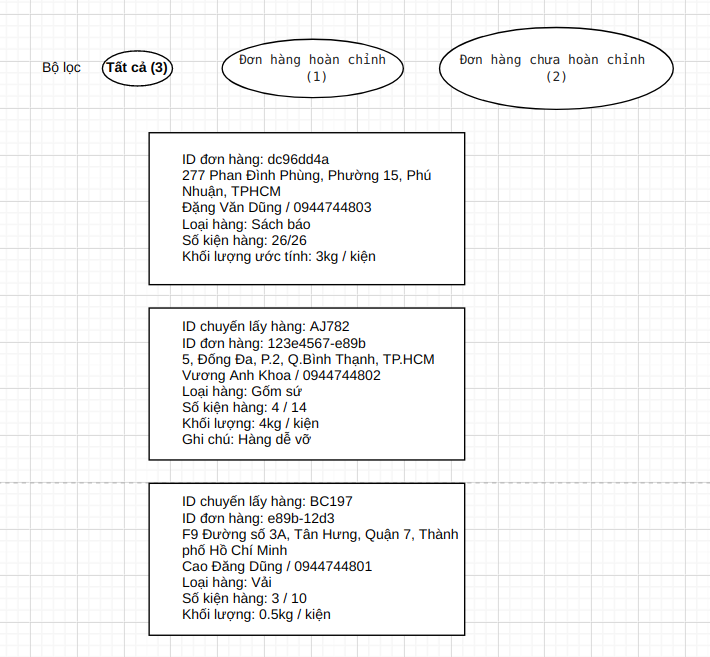
\includegraphics[width=0.75\textwidth]{/hangtrongkho.png}
			\centering
			\linebreak
			\caption{Wireframe xem danh sách hàng trong kho của thủ kho}
		\end{figure}
		
		\item \textbf{Xác nhận kiện hàng vào kho}:
		Khi tài xế nội tỉnh đến kho, thủ kho sẽ search ID của tài xế để xem list kiện hàng được phân công của tài xế Thủ kho sẽ kiểm tra xe của tài xế và check vào những kiện hàng thật sự có trong xe để hoàn tất quá trình nhập kho của kiện hàng. (Tức hệ thống sẽ cập nhật số kiện hàng đã vào kho của đơn hàng). Trạng thái đơn hàng cập nhật từ <Đang lấy hàng>  -->  <Đã vào kho tập trung 1>  nếu tất cả các kiện hàng của đơn đã được check vào kho. 
		
		\begin{figure}[!ht]
			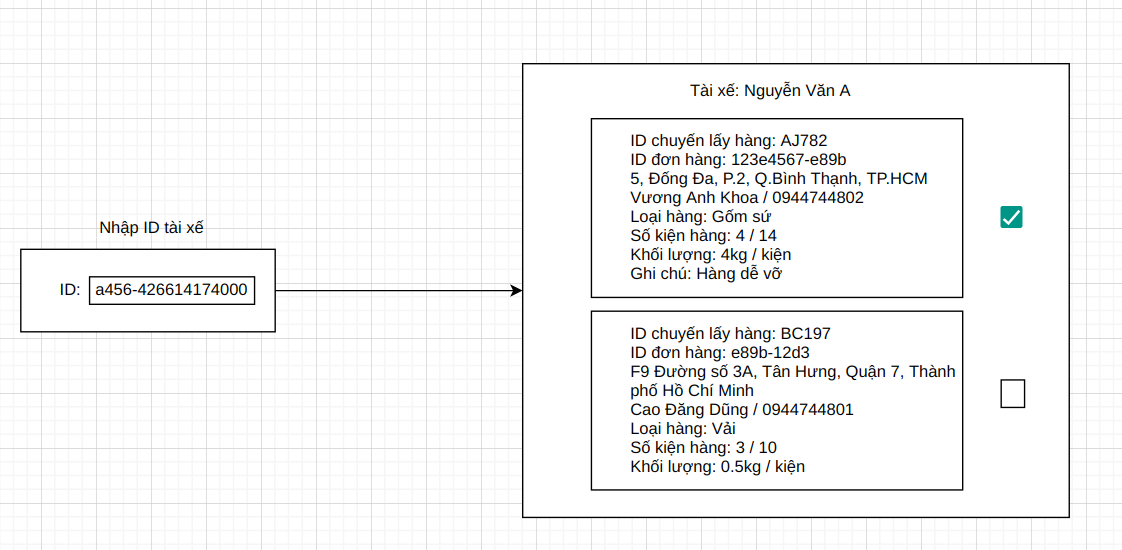
\includegraphics[width=1\textwidth]{/xacnhankienhangvaokho.png}
			\centering
			\linebreak
			\caption{Wireframe xác nhận kiện hàng vào kho}
		\end{figure}
		
		\item \textbf{Xác nhận đơn hàng xuất kho}: Khi tài xế liên tỉnh xuất kho đến yêu cầu thủ kho những đơn hàng cần giao liên tỉnh thì thủ kho sẽ search ID của tài xế liên tỉnh đó và xem được list các đơn hàng mà tài xế liên tỉnh đó được phân phối. Khi tài xế liên tỉnh chuyển những đơn hàng đó lên xe liên tỉnh thì thủ kho sẽ check vào những kiện hàng sẽ lên xe để hoàn tất quá trình xuất kho của kiện hàng. Việc check như vậy sẽ cập nhật trạng thái của đơn hàng trên hệ thống (Đã vào kho tập trung 1 -> Đang giao liên tỉnh).
		\item \textbf{Xác nhận đơn hàng vào kho}: Khi tài xế liên tỉnh đến kho, thủ kho sẽ search ID của tài xế liên tỉnh để xem list đơn hàng được phân công của tài xế Thủ kho sẽ kiểm tra xe của tài xế và check vào những đơn hàng thật sự có trong xe để hoàn tất quá trình nhập kho của đơn hàng.Trạng thái đơn hàng cập nhật từ (Đang giao liên tỉnh -> Đã vào kho tập trung 2). Nếu người gửi chọn option tự gửi đến kho, thủ kho sẽ search ID của người gửi và thực hiện tiếp các bước như trên. 
		
		\newpage
		
		\begin{figure}[!ht]
			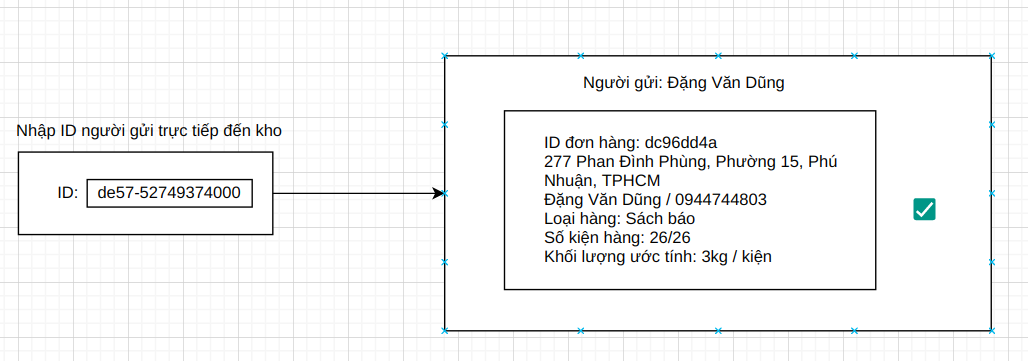
\includegraphics[width=1\textwidth]{/xacnhandonhangvaokho.png}
			\centering
			\linebreak
			\caption{Wireframe xác nhận đơn hàng vào kho}
		\end{figure}
		
		\item \textbf{Xác nhận kiện hàng xuất kho}: Khi tài xế nội tỉnh đến yêu cầu thủ kho những kiện hàng cần giao nội tỉnh thì thủ kho sẽ search ID của tài xế nội tỉnh đó và xem được list các kiện hàng mà tài xế nội tỉnh đó được phân phối. Khi tài xế nội tỉnh chuyển những kiện hàng đó lên xe nội tỉnh thì thủ kho sẽ check những kiện hàng trong list xem ở trên để xác nhận việc tài xế nội tỉnh đã chất hàng lên xe. Việc check như vậy sẽ cập nhật trạng thái của đơn hàng trên hệ thống (Đã vào kho tập trung 2 -> Đang giao hàng (x/tổng số kiện)).
	\end{itemize}
	\subsection{Hệ thống thông báo}
	\textbf{Gửi thông báo đến mail người dùng cho mỗi mức chuyển trạng thái}: Hệ thống sẽ gửi mail đến người dùng mỗi khi đơn hàng chuyển qua một trạng thái
	
	\begin{figure}[!ht]
		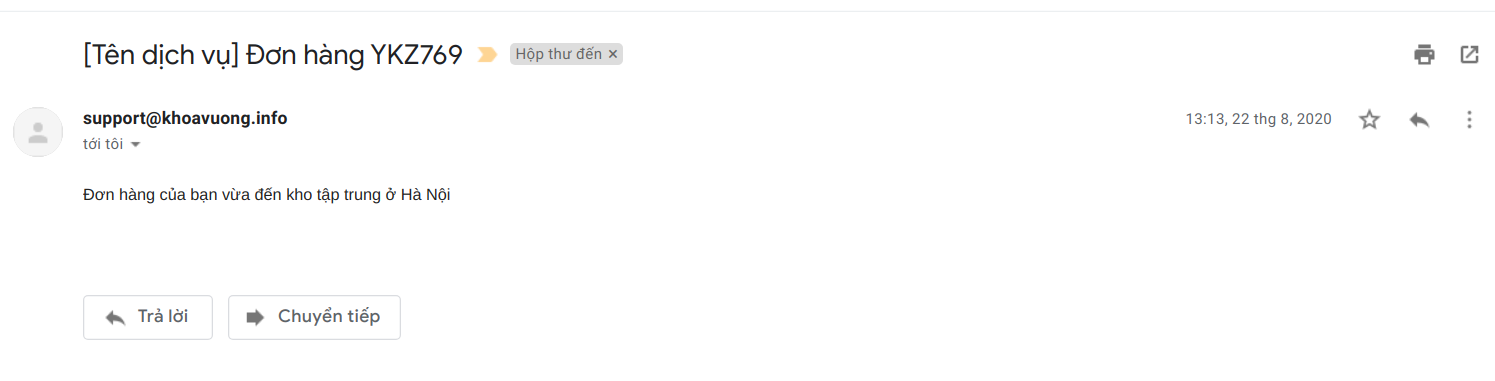
\includegraphics[width=1\textwidth]{/mail.png}
		\centering
		\linebreak
		\caption{Ví dụ mail thông báo dự kiến khi đơn hàng chuyển trạng thái}
	\end{figure}
	
\end{itemize}